% Created 2018-11-30 Fri 08:51
% Intended LaTeX compiler: pdflatex
\documentclass[presentation]{beamer}
\usepackage[utf8]{inputenc}
\usepackage[T1]{fontenc}
\usepackage{graphicx}
\usepackage{grffile}
\usepackage{longtable}
\usepackage{wrapfig}
\usepackage{rotating}
\usepackage[normalem]{ulem}
\usepackage{amsmath}
\usepackage{textcomp}
\usepackage{amssymb}
\usepackage{capt-of}
\usepackage{natbib}
\usepackage[linktocpage,pdfstartview=FitH,colorlinks,
linkcolor=blue,anchorcolor=blue,
citecolor=blue,filecolor=blue,menucolor=blue,urlcolor=blue]{hyperref}
\setbeamertemplate{frame footer}{\insertshortauthor}
\setbeamerfont{page number in head/foot}{size=\tiny}
\setbeamercolor{footline}{fg=gray}
\usepackage{amsmath}
\author{Florian Hollenbach}
\usepackage[english]{isodate}
\usepackage{amsmath,amsthm,amssymb,amsfonts}
\newcommand{\E}{\mathbb{E}}
\newcommand{\V}{\mathbb{V}}
\usetheme{metropolis}
\usecolortheme{}
\usefonttheme{}
\useinnertheme{}
\useoutertheme{}
\author{Florian Hollenbach}
\date{\today}
\title{Political Science 209 - Fall 2018}
\subtitle{Hypothesis Testing}

\hypersetup{
 pdfauthor={Florian Hollenbach},
 pdftitle={Political Science 209 - Fall 2018},
 pdfkeywords={},
 pdfsubject={},
 pdfcreator={Emacs 25.3.1 (Org mode 9.1.14)}, 
 pdflang={English}}
\begin{document}

\maketitle



\begin{frame}[label={sec:org004359b}]{Hypothesis Testing}
Goal: Try to determine whether result is due to chance or not

Method: ``\emph{Proof}'' by contradiction

We try to reject the \emph{null hypothesis}
\end{frame}

\begin{frame}[label={sec:org4cc7377}]{Hypothesis Testing}
Generally we have two hypotheses:

1.\(H_{0}\) Null hypothesis: no relationship

2.\(H_{1}\) Alternative hypothesis: complement to null hypothesis: expected relationship
\end{frame}

\begin{frame}[label={sec:orgd9d3bff}]{Hypothesis Testing}
We can \alert{never} prove a hypothesis to be true or reject a hypothesis with certainty

Instead, we may \alert{fail to reject the null}

We use data and statistical test to infer whether we can \emph{reject or fail to reject the null}
\end{frame}


\begin{frame}[label={sec:org075add4}]{Hypothesis Testing}
\begin{center}
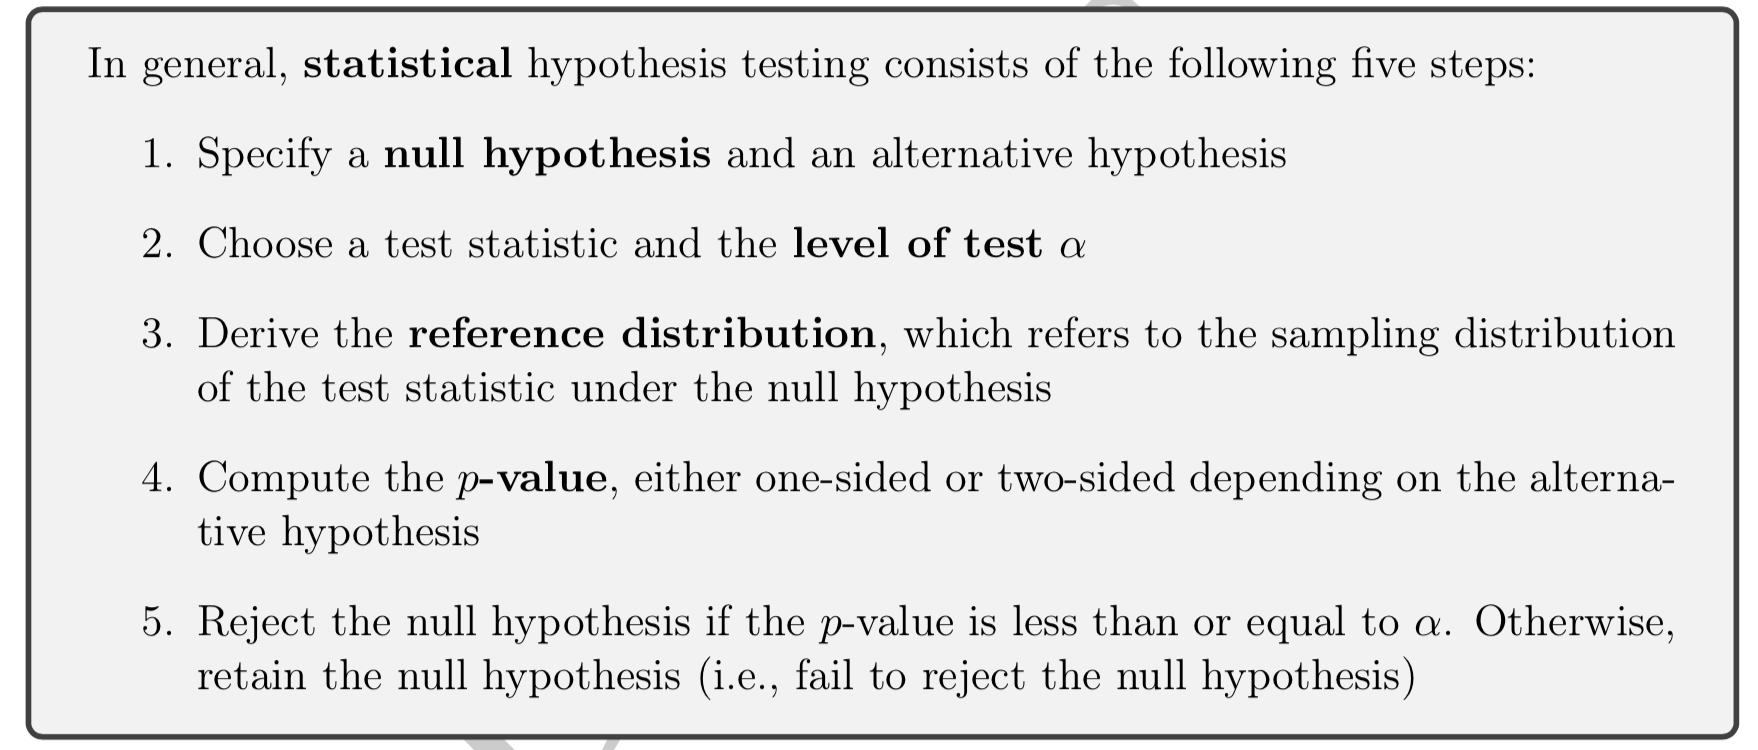
\includegraphics[width=9cm]{/Users/florianhollenbach/Documents/GitHub/Polisci209_2018/slides/week14/hyp.png}
\end{center}
\end{frame}
\end{document}